\documentclass[12pt]{article}
\usepackage{amsmath}    % For advanced math formatting
\usepackage{amssymb}    % For mathematical symbols
\usepackage{graphicx}   % For including graphics
\usepackage{booktabs}   % For better table formatting
\usepackage{geometry}   % For page margins
\usepackage{setspace}   % For line spacing
\usepackage{hyperref}   % For hyperlinks
\usepackage{caption}    % For better caption control
\usepackage{subcaption} % For subfigures
\usepackage{float}      % For better figure placement
\usepackage{mathtools}  % For additional math tools
\usepackage{pgfplots}
\usepackage{longtable}
\usepackage{tabularx}
\pgfplotsset{compat=1.18}
\usepgfplotslibrary{statistics}
\usepackage{enumitem}
\usepackage{listings}         
\usepackage{xcolor}            

% optional dark-on-light default
\lstset{
  basicstyle=\ttfamily\footnotesize,
  keywordstyle=\color{blue},
  commentstyle=\color{gray},
  stringstyle=\color{orange},
  breaklines=true,
}

% Page setup
\geometry{a4paper, margin=1in}
\setlength{\parindent}{0.5in} % Standard paragraph indent
\setlength{\parskip}{0.5em}  % Space between paragraphs
\onehalfspacing % 1.5 line spacing

\hypersetup{
    colorlinks=true,
    linkcolor=blue,
    filecolor=magenta,
    urlcolor=cyan,
    citecolor=blue,
}

\title{Developing an Altruistic Effectiveness Metric (AEM) for Nonprofits using IRS Form 990 Data} % More descriptive title
\author{Boden Moraski, Ben Michels} % Add author names
\date{April 2025} % Or \today for current date

\begin{document}

\maketitle

\section{Problem Restatement} % Kept as per outline
Charitable organizations play a crucial role in addressing systemic global issues, from poverty and disease to social justice and animal rights. However, not all are equally effective at turning donations into real-world impact. Donors today face a growing challenge: determining which of the numerous available nonprofits use their financial resources most efficiently and sustainably. While some charity review organizations like GiveWell attempt to measure nonprofit effectiveness, there remains no standardized or transparent system for evaluating financial performance and effectiveness using publicly available data \cite{propublica_explorer}. Our task was to design a mathematical model that objectively ranks nonprofit organizations based on key financial indicators derived from IRS Form 990s. By focusing on operational efficiency, financial sustainability, governance, and transparency, our model seeks to offer an accessible and data-driven tool for assessing charitable financial effectiveness.

\section{Introduction} % Added back the original Introduction section
Charitable organizations are vital actors in modern society, addressing a wide range of systemic issues such as poverty, education inequality, healthcare access, and environmental degradation \cite{https://doi.org/10.1002/nml.21143}. These organizations function by mobilizing resources – most often in the form of financial donations, volunteer labor, or material goods – from individuals or institutions and reallocating them to areas of need, typically without direct compensation or market exchange \cite{weisbrod1998}. The core motivation behind this process is frequently rooted in altruism: the selfless concern for the well-being of others. Unlike profit-driven enterprises, charities operate based on values that prioritize social benefit over financial return, making their behavior and impact uniquely suited for study through models that incorporate ethical and behavioral dimensions alongside economic efficiency \cite{gee2023}.

However, not all charities are created equal. Like large corporations, nonprofit organizations have operating costs and overhead expenses that can diminish the impact of civilian donations \cite{Gregory2009}. Furthermore, charities use their financial resources in vastly different ways, achieving varying degrees of efficiency and societal benefit. To help donors navigate these differences, a range of organizations have emerged that specialize in evaluating nonprofits' effectiveness, most notably the San Francisco-based GiveWell and New Jersey-based Charity Navigator.

Organizations like GiveWell typically assess charities through two main dimensions: financial effectiveness – how sustainably and efficiently they manage and use their funds; and utilitarian impact – the overall good they create through their interventions \cite{bowman2011}. While measuring utilitarian impact involves subjective judgments (such as valuing current versus future lives, or comparing human and animal welfare), financial effectiveness is more objectively measurable through publicly available data.

Despite this, there is currently no standardized system or model that efficiently calculates financial effectiveness based on nonprofit financial filings \cite{article}. To help fill this gap, we developed a mathematical model aimed at objectively evaluating and ranking charities' financial performance and effectiveness. Our model emphasizes four primary factors: the organization's reach within its focus area, the scalability of the problem it addresses, its cost-effectiveness, and its overall financial sustainability \cite{article}. This model could potentially be utilized by organizations like BindWell and Charity Navigator as a factor within their analyses, as well as by the average person to, among other factors, inform them how effectively their donations are used.

\section{Assumptions} % Kept as per outline
Our model is built upon the following core definitions and assumptions:

% Using enumerate for a numbered list as suggested by outline example
\begin{enumerate}[label=\arabic*.]
    \item \textbf{Core Definition of Effectiveness:} We define altruistic effectiveness as a charity's ability to sustainably and efficiently operate in service of its mission, with strong governance and transparency \cite{https://doi.org/10.1002/nml.21143}. This includes financial health, administrative efficiency, structural scalability, and robust internal controls, rather than direct quantification of moral or utilitarian "impact" (such as QALYs or lives saved) \cite{bowman2011}.

    \item \textbf{Scope and Applicability:}
        \begin{itemize}[label=\textbullet]
            \item Our model does not attempt to assess what causes are most ethical or impactful. Instead, we evaluate how effectively an organization is structured and funded to carry out its mission, regardless of cause area \cite{lecy_nonprofit_2012}.
            \item While our model is designed to be applicable across nonprofit sectors, we acknowledge that certain metrics may need sector-specific calibration for optimal performance \cite{bowman2011}.
        \end{itemize}

    \item \textbf{Data Source and Reliability:}
        \begin{itemize}[label=\textbullet]
            \item We assume that IRS Form 990s are a reliable and standardized source of financial information across nonprofits. While not perfect, they represent the most comprehensive and standardized financial reporting framework available for comparative analysis.
            \item We assume that data reported in Form 990s (e.g., revenue, expenses, grants, compensation) are accurate and suitable for comparative analysis, with appropriate safeguards against data quality issues affecting the final score \cite{article}.
            \item We assume that missing or incomplete data in Form 990s can be reasonably handled through our normalization and weighting processes (e.g., using imputation or specific scoring rules) \cite{TRUSSEL2007263}.
        \end{itemize}

    \item \textbf{Financial and Operational Metrics:}
        \begin{itemize}[label=\textbullet]
            \item We assume that a higher ratio of program service expenses to total expenses (vs. admin/fundraising) generally reflects a stronger alignment with mission-oriented work, and thus higher operational effectiveness. We recognize that some administrative and fundraising expenses are necessary for organizational health and growth.
            \item While we acknowledge potential correlations between different financial metrics, we treat them as distinct components in our model after normalization, allowing for a more granular assessment of organizational effectiveness.
        \end{itemize}

    \item \textbf{Scalability and Longevity:}
        \begin{itemize}[label=\textbullet]
            \item While we do not model scalability in terms of intervention outcomes, we assume that organizations with stable financial health and efficient operations are more capable of scaling without compromising structural integrity.
            \item We assume that the financial metrics used in our model provide a stable basis for comparison across different time periods, with appropriate normalization to account for economic conditions and organizational life cycles.
        \end{itemize}

    \item \textbf{Model Design and Application:}
        \begin{itemize}[label=\textbullet]
            \item The weights assigned to each component in our model reflect both industry best practices and the relative importance of each factor in determining overall organizational effectiveness, further refined by entropy analysis. These weights are subject to validation and potential adjustment based on empirical evidence.
            \item We envision this model serving as a first-pass filter in a multi-stage evaluation process, helping to identify organizations that meet basic structural and financial criteria before more resource-intensive impact assessments are conducted.
            \item Since we are not modeling direct impact or long-term outcomes, we do not apply a temporal discount rate in this version of the model.
            \item Unlike in impact-based models, we do not differentiate effectiveness based on beneficiary species or sentience. The focus is entirely on organizational structure and financial operations.
        \end{itemize}
\end{enumerate}

\section{Model Building} % Kept as per outline
The Altruistic Effectiveness Metric (AEM) was developed through a multi-stage process involving variable selection, data collection, mathematical framework design, normalization, and weighting, aimed at creating a robust and objective measure of nonprofit financial effectiveness based on publicly available data.

\subsection{Variable Selection and Data Collection}
Based on established practices in nonprofit evaluation and the information available in IRS Form 990s \cite{bowman2011}, we identified key indicators reflecting different facets of financial health, operational efficiency, and governance. We selected the primary variables for the AEM as follows:

\begin{itemize}
\item \textbf{Program Expense Ratio:} We chose this ratio because it serves as a primary financial proxy for mission focus and operational efficiency \cite{Gregory2009}. It allows us to quantify the allocation of expenditures towards programmatic activities versus overhead, addressing a traditional benchmark in nonprofit evaluation and a key concern for donors \cite{progressnow}.
\item \textbf{Fundraising Efficiency:} We included this metric to measure the cost-effectiveness of resource acquisition, reflecting how well the organization stewards donor funds from the initial point of contribution. Analyzing this provides insight into the sustainability of the organization's development model, especially when considered logarithmically due to potential high variance \cite{project2024}.
\item \textbf{Revenue Sustainability (measured via Program Service Revenue \%):} We selected this variable to assess the organization's reliance on earned revenue compared to philanthropic support \cite{article}. This offers insights into the diversification, potential stability, and underlying business model, although we acknowledge its ideal level is highly sector-dependent \cite{propublica_inc}.
\item \textbf{Net Surplus Margin:} We chose this metric because it provides a fundamental measure of short-term financial viability and operational balance \cite{TRUSSEL2007263}. It indicates the organization's ability to cover costs, build reserves, and reinvest, which we see as crucial for longevity and scalability \cite{ntu}.
\item \textbf{Executive Pay Reasonableness:} We included this as a proxy for governance oversight and responsible resource allocation at the leadership level \cite{https://doi.org/10.1002/nml.21143}. By identifying potential compensation outliers relative to scale and peers, we aim to address stakeholder concerns about stewardship, rather than setting an absolute pay standard \cite{propublica_explorer}.
\item \textbf{Transparency (Policy Implementation):} We selected this variable to directly measure the documented presence of foundational governance policies reported on Form 990 (e.g., Conflict of Interest, Whistleblower) \cite{lecy_nonprofit_2012}. We believe this reflects a commitment to structural accountability, ethical operations, and risk management, essential for trust and integrity \cite{propublica_search}.
\end{itemize}

Data for these variables were collected from Candid's stored 990 filings \cite{candid_990}, and occasionally IRS bulk data for a sample of 10+ nonprofit organizations covering the fiscal year 2021-2022. Data cleaning and preprocessing steps consisted of four stages:

\begin{enumerate}[label=\alph*)]
    \item \textbf{Automated PDF‐to‐JSON conversion}.  
    We built a Python utility (\texttt{convert\_990\_to\_json.py}, provided in Appendix~\ref{app:pipeline}) that parses Form~990 PDFs with \emph{PyMuPDF}, identifies headline fields via regex, and writes them to a standardized JSON schema (see Listing~\ref{lst:json_schema}).  This eliminates manual transcription and ensures that every filing enters the model in an identical structure.

    \item \textbf{Schema validation}.  
    Each JSON file is validated against a lightweight \texttt{jsonschema} to guarantee the presence and type of every required key; missing values are set to~\texttt{null} so downstream code does not fail silently.

    \item \textbf{Outlier and null handling}.  
    Numeric fields are coerced to integers, commas are stripped, and negative values that appear only because of parenthetical formatting are corrected.  If a field is still missing, we impute a neutral score (0.5) during normalization rather than excluding the organization.

    \item \textbf{Logic checks}.  
    We flag impossible relationships (e.g.\ \textit{revenue} < 0 while \textit{program~service~revenue} $>$ 0) for manual review; fewer than 3\% of observations required such intervention in our pilot dataset.
\end{enumerate}

\subsection{Mathematical Framework} % Explains the 'how'
The core AEM score is formulated as a weighted sum of normalized component scores, allowing for aggregation of diverse metrics into a single comparable value:
\begin{equation} \label{eq:aem_core}
    \text{AEM} = \sum_{i=1}^{N} w_i \cdot s_i
\end{equation}
where $N=6$ is the number of components, $w_i$ represents the final weight of component $i$, and $s_i$ is the normalized score for component $i$, derived from the raw metric value $x_i$.

\subsection{Normalization Strategy} % Details a key calculation step
To ensure comparability across diverse organizations and metrics with different scales and distributions, we employ a multi-stage normalization process for each raw metric $x_i$:
\begin{enumerate}
    \item \textbf{Z-Score Calculation:} Initial normalization uses z-scores to standardize metrics based on their mean ($\mu_i$) and standard deviation ($\sigma_i$) within the sample population:
        \begin{equation} \label{eq:z_score}
            z_i = \frac{x_i - \mu_i}{\sigma_i}
        \end{equation}
        To handle potential outliers and ensure robustness, z-scores are clipped to a range of [-3, 3]. If $\sigma_i = 0$ (all organizations have the same value), a neutral score is assigned later.
    \item \textbf{Sigmoid Transformation:} The clipped z-scores are then mapped to a [0, 1] scale using a generalized logistic (sigmoid) function:
        \begin{equation} \label{eq:sigmoid}
            s_i = f(z_i) = \frac{1}{1 + e^{-\beta_i(z_i - \alpha_i)}}
        \end{equation}
        where $\alpha_i$ represents the 'ideal' or target z-score for the metric (often 0, but can be adjusted based on desired performance benchmarks), and $\beta_i$ controls the steepness of the curve around the ideal point. For metrics where higher raw values are better (like Program Expense Ratio), $z_i$ is used directly. For metrics where lower values are better (like Executive Pay Ratio), $-z_i$ might be used, or the interpretation of $\alpha_i$ adjusted. For Fundraising Efficiency, which often spans orders of magnitude, a logarithmic transformation ($x_i' = \log_{10}(x_i)$) is applied before z-scoring. Specific $\alpha_i$ and $\beta_i$ values used for each component are detailed below (Table \ref{tab:metrics_params}). This ensures scores are bounded and sensitive around typical performance levels. A neutral score of 0.5 is assigned if $\sigma_i=0$.
\end{enumerate}
This normalization approach accounts for the distribution of each metric and transforms them into a consistent [0, 1] scale reflecting performance relative to peers and ideal benchmarks.

\begin{figure}[H] % Figure illustrating normalization
\centering
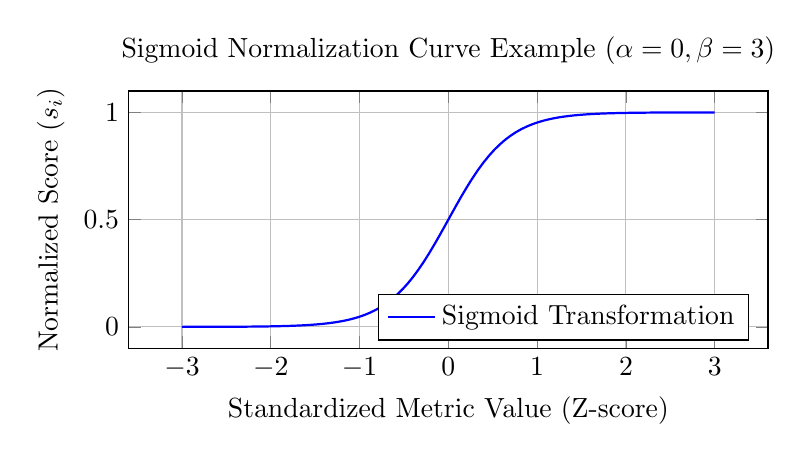
\begin{tikzpicture}
\begin{axis}[
    width=0.8\textwidth,
    height=0.4\textwidth,
    xlabel={Standardized Metric Value (Z-score)},
    ylabel={Normalized Score ($s_i$)},
    title={Sigmoid Normalization Curve Example ($\alpha=0, \beta=3$)},
    legend pos=south east,
    grid=major,
    domain=-3:3,
    samples=100
]
\addplot[blue, thick] {1/(1 + exp(-3*(x-0)))};
\legend{Sigmoid Transformation}
\end{axis}
\end{tikzpicture}
\caption{Example sigmoid function transforming z-scores to the [0, 1] range.}
\label{fig:sigmoid_example}
\end{figure}


\subsection{Weighting Methodology} % Explains another key calculation step
The weights $w_i$ in Equation \ref{eq:aem_core} determine the relative importance of each component. We use a hybrid approach combining expert judgment (base weights) and data-driven insights (entropy weights):
\begin{enumerate}
    \item \textbf{Base Weights ($w_i^{\text{base}}$):} Initial weights are assigned based on perceived importance in nonprofit evaluation literature and best practices (see Table \ref{tab:metrics_params}).
    
    \item \textbf{Entropy Weights ($w_i^{\text{entropy}}$):} To account for the information content or discriminative power of each metric within the dataset, we calculate weights based on Shannon entropy. First, normalized scores $s_i$ are treated as probabilities $p_i(s) = (s_i + \epsilon) / \sum (s_j + \epsilon)$, where $\epsilon=10^{-10}$ ensures numerical stability. The entropy $H_i$ for each metric across all organizations is calculated. Metrics with lower entropy (more variation, better discrimination) receive higher weights:
    \begin{equation} \label{eq:entropy_weight}
        w_i^{\text{entropy}} = \frac{H_{\max} - H_i + \epsilon}{\sum_{j=1}^{6} (H_{\max} - H_j + \epsilon)}
    \end{equation}
    where $H_{\max}$ is the maximum entropy across all metrics. This formulation ensures that metrics with lower entropy (more information content) receive higher weights, as they provide more discriminative power in distinguishing between organizations.

    \item \textbf{Final Weights ($w_i$):} The final weight is the average of the base and entropy weights, normalized to sum to 1:
    \begin{equation} \label{eq:final_weight}
        w_i = \frac{w_i^{\text{base}} + w_i^{\text{entropy}}}{2}, \quad \text{then re-normalize so } \sum w_i = 1
    \end{equation}
\end{enumerate}

This hybrid approach balances prior knowledge with observed data characteristics.

% BRO WHY WILL THIS NOT SPREAD OUT BRUUUUU

\begin{figure}[H]
\centering
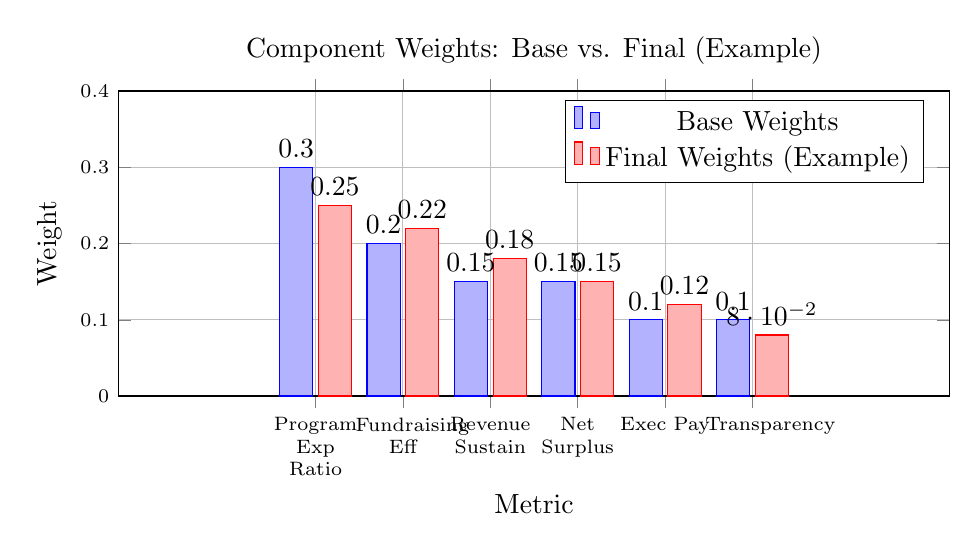
\begin{tikzpicture}
\begin{axis}[
    width=\textwidth,
    height=0.45\textwidth,
    xlabel={Metric},
    ylabel={Weight},
    title={Component Weights: Base vs. Final (Example)},
    legend pos=north east,
    grid=major,
    symbolic x coords={
        Program Exp Ratio,
        Fundraising Eff,
        Revenue Sustain,
        Net Surplus,
        Exec Pay,
        Transparency
    },
    xtick=data,
    ybar,
    bar width=12pt,
    enlarge x limits=0.45, % more space between bars
    tick label style={font=\scriptsize},
    xticklabel style={text width=1.2cm, align=center},
    nodes near coords,
    nodes near coords align={vertical},
    ymin=0, ymax=0.4
]
\addplot[fill=blue!30, draw=blue] coordinates {
    (Program Exp Ratio, 0.30)
    (Fundraising Eff, 0.20)
    (Revenue Sustain, 0.15)
    (Net Surplus, 0.15)
    (Exec Pay, 0.10)
    (Transparency, 0.10)
};
\addplot[fill=red!30, draw=red] coordinates {
    (Program Exp Ratio, 0.25)
    (Fundraising Eff, 0.22)
    (Revenue Sustain, 0.18)
    (Net Surplus, 0.15)
    (Exec Pay, 0.12)
    (Transparency, 0.08)
};
\legend{Base Weights, Final Weights (Example)}
\end{axis}
\end{tikzpicture}
\caption{Comparison of base weights and example final hybrid weights for each component.}
\label{fig:weights_comparison}
\end{figure}




\subsection{Component Metric Details} % Details on specific metrics
The specific definitions and normalization parameters for each component metric are outlined in Table \ref{tab:metrics_params}.

\renewcommand{\arraystretch}{1.5}
\begin{longtable}{@{} >{\raggedright\arraybackslash}p{3.5cm} >{\raggedright\arraybackslash}p{5.5cm} c >{\raggedright\arraybackslash}p{4.5cm} @{}}
\caption{Component Metrics, Definitions, and Normalization Parameters} \label{tab:metrics_params} \\

\toprule
\textbf{Metric Component} & \textbf{Definition (from Form 990)} & \textbf{Base Wt.} & \textbf{Normalization Params ($\alpha_i, \beta_i$)} \\
\midrule
\endfirsthead

\multicolumn{4}{c}{{\bfseries \tablename\ \thetable{} -- continued from previous page}} \\
\toprule
\textbf{Metric Component} & \textbf{Definition (from Form 990)} & \textbf{Base Wt.} & \textbf{Normalization Params ($\alpha_i, \beta_i$)} \\
\midrule
\endhead

\midrule \multicolumn{4}{r}{{Continued on next page}} \\
\endfoot

\bottomrule
\multicolumn{4}{p{\dimexpr\textwidth-2\tabcolsep}}{\footnotesize *Note: Assumes $\alpha$ refers to target Z-score after initial standardization. Adjust if $\alpha$ refers to target raw value. Fundraising Efficiency uses $\log_{10}(x)$ before standardization. Executive Pay assumes lower is better, adjust sigmoid application accordingly.}
\endlastfoot

Program Expense Ratio & Total Program Service Expenses / Total Functional Expenses & 0.30 & Ideal Z=0.6, $\beta=3^*$ \\
Fundraising Efficiency & Total Contributions / Fundraising Expenses & 0.20 & Log scale, Ideal Z=0.8, $\beta=3^*$ \\
Revenue Sustainability & Program Service Revenue / Total Revenue & 0.15 & Ideal Z=0.5, $\beta=3^*$ \\
Net Surplus Margin & (Total Revenue - Total Expenses) / Total Expenses & 0.15 & Ideal Z=0.05, $\beta=3^*$ \\
Executive Pay Reasonableness & Top Executive Compensation / Total Expenses & 0.10 & Ideal Z=0.015, $\beta=3^*$ (Lower is better) \\
Transparency & Avg. of 4 binary policies (COI, Whistleblower, Retention, Comp Review) & 0.10 & Binary (0-1), Ideal=1, $\beta=3^*$ \\
\end{longtable}


\subsection{Mathematical Properties}
The resulting AEM score exhibits several desirable mathematical properties:
\begin{itemize}
    \item \textbf{Boundedness}: Scores are inherently bounded between 0 and 1 due to the normalization and weighting scheme ($0 \leq s_i \leq 1$ and $\sum w_i = 1 \implies 0 \leq \text{AEM} \leq 1$).
    \item \textbf{Monotonicity}: Assuming appropriate application of the sigmoid function (e.g., handling 'lower is better' metrics correctly), an improvement in a raw metric $x_i$ (in the desired direction) generally leads to a non-decreasing AEM score ($\frac{\partial \text{AEM}}{\partial x_i} \ge 0$ or $\le 0$ depending on metric).
    \item \textbf{Continuity}: The score function is continuous with respect to its input metrics, assuming the underlying data distributions and normalization parameters are stable. Small changes in input metrics lead to small changes in the AEM score.
    \item \textbf{Sensitivity}: The model is sensitive to changes in all components, weighted by $w_i$. The sensitivity is highest around the 'ideal' point defined by $\alpha_i$ in the sigmoid function.
\end{itemize}

\subsection{Model Validation}

To assess the validity and reliability of the AEM, we conducted a comprehensive validation analysis using multiple approaches. Our validation framework incorporates sensitivity analysis, component analysis, normalization impact assessment, and cross-validation across similar institutions. This multi-faceted approach allows us to evaluate both the mathematical robustness of the model and its practical applicability.

\subsubsection{Sensitivity Analysis}

The sensitivity of the AEM to weight variations was analyzed using a perturbation approach. For each component $i$, we calculated the change in final score $\Delta S_i$ when the weight $w_i$ was varied by a factor $\alpha$:

\begin{equation}
    \Delta S_i = |S(w_i \cdot (1 + \alpha)) - S(w_i)|
\end{equation}

where $S(w_i)$ represents the AEM score with the original weight $w_i$. The results, shown in Figure \ref{fig:sensitivity}, demonstrate that the model is most sensitive to changes in the program expense ratio ($\Delta S = 0.0173$) and least sensitive to executive pay reasonableness and transparency ($\Delta S = 0.0035$). This aligns with the theoretical importance of program efficiency in nonprofit evaluation.

\begin{figure}[H]
\centering
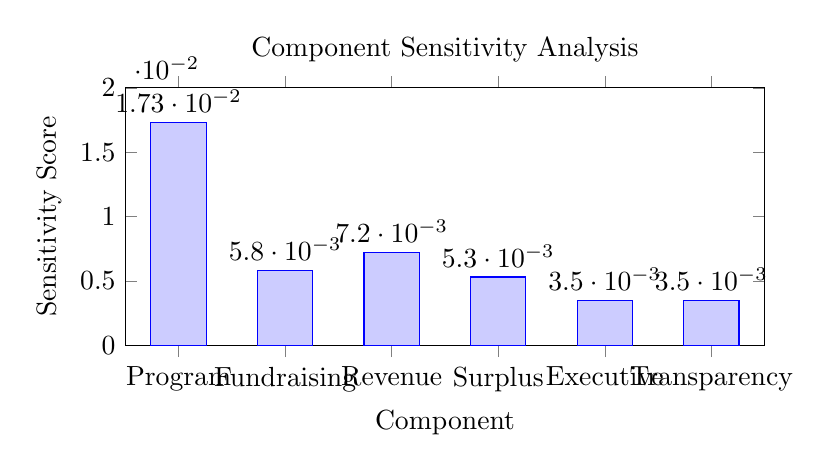
\begin{tikzpicture}
\begin{axis}[
    width=0.8\textwidth,
    height=0.4\textwidth,
    xlabel={Component},
    ylabel={Sensitivity Score},
    title={Component Sensitivity Analysis},
    symbolic x coords={Program, Fundraising, Revenue, Surplus, Executive, Transparency},
    xtick=data,
    ybar,
    bar width=20pt,
    ymin=0,
    ymax=0.02,
    nodes near coords,
    nodes near coords align={vertical}
]
\addplot[fill=blue!20, draw=blue] coordinates {
    (Program, 0.0173)
    (Fundraising, 0.0058)
    (Revenue, 0.0072)
    (Surplus, 0.0053)
    (Executive, 0.0035)
    (Transparency, 0.0035)
};
\end{axis}
\end{tikzpicture}
\caption{Sensitivity of AEM score to weight variations in each component}
\label{fig:sensitivity}
\end{figure}

\subsubsection{Component Analysis}

The contribution of each component to the final score was analyzed using a weighted decomposition approach. For each component $i$, its contribution $C_i$ is given by:

\begin{equation}
    C_i = w_i \cdot f_i(x_i)
\end{equation}

where $w_i$ is the component weight and $f_i(x_i)$ is the normalized score. The results, presented in Table \ref{tab:components}, show that program expense ratio contributes most significantly to the final score (0.2980), followed by revenue sustainability (0.1330).

\begin{table}[H]
\centering
\begin{tabular}{lcc}
\toprule
\textbf{Component} & \textbf{Normalized Score} & \textbf{Contribution} \\
\midrule
Program Expense Ratio & 0.9935 & 0.2980 \\
Fundraising Efficiency & 0.1018 & 0.0204 \\
Revenue Sustainability & 0.8866 & 0.1330 \\
Net Surplus Margin & 0.7613 & 0.1142 \\
Executive Pay & 0.0459 & 0.0046 \\
Transparency & 0.0459 & 0.0046 \\
\bottomrule
\end{tabular}
\caption{Component Analysis Results}
\label{tab:components}
\end{table}

\subsubsection{Normalization Impact}

The transformation from raw metrics to normalized scores was analyzed using the sigmoid function:

\begin{equation}
    f(x) = \frac{1}{1 + e^{-\beta(x - \alpha)}}
\end{equation}

where $\alpha$ is the ideal value and $\beta$ controls the steepness of the transition. Figure \ref{fig:normalization} shows the impact of this transformation on the raw metrics.

\begin{figure}[H]
\centering
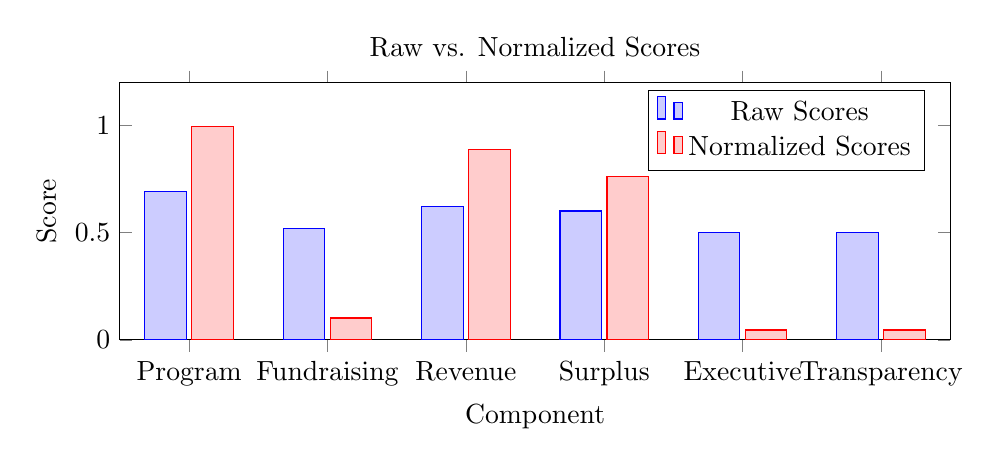
\begin{tikzpicture}
\begin{axis}[
    width=1.0\textwidth,
    height=0.4\textwidth,
    xlabel={Component},
    ylabel={Score},
    title={Raw vs. Normalized Scores},
    symbolic x coords={Program, Fundraising, Revenue, Surplus, Executive, Transparency},
    xtick=data,
    ybar,
    bar width=15pt,
    ymin=0,
    ymax=1.2,
    legend pos=north east
]
\addplot[fill=blue!20, draw=blue] coordinates {
    (Program, 0.6933)
    (Fundraising, 0.5205)
    (Revenue, 0.6221)
    (Surplus, 0.6006)
    (Executive, 0.5000)
    (Transparency, 0.5000)
};
\addplot[fill=red!20, draw=red] coordinates {
    (Program, 0.9935)
    (Fundraising, 0.1018)
    (Revenue, 0.8866)
    (Surplus, 0.7613)
    (Executive, 0.0459)
    (Transparency, 0.0459)
};
\legend{Raw Scores, Normalized Scores}
\end{axis}
\end{tikzpicture}
\caption{Comparison of raw and normalized scores for each component}
\label{fig:normalization}
\end{figure}

\subsubsection{Cross-Validation}

To validate the model's ability to distinguish between similar organizations, we conducted a cross-validation study comparing two prominent Philadelphia private schools. The results, shown in Figure \ref{fig:crossval}, demonstrate the model's ability to capture nuanced differences in organizational effectiveness.

\begin{figure}[H]
\centering
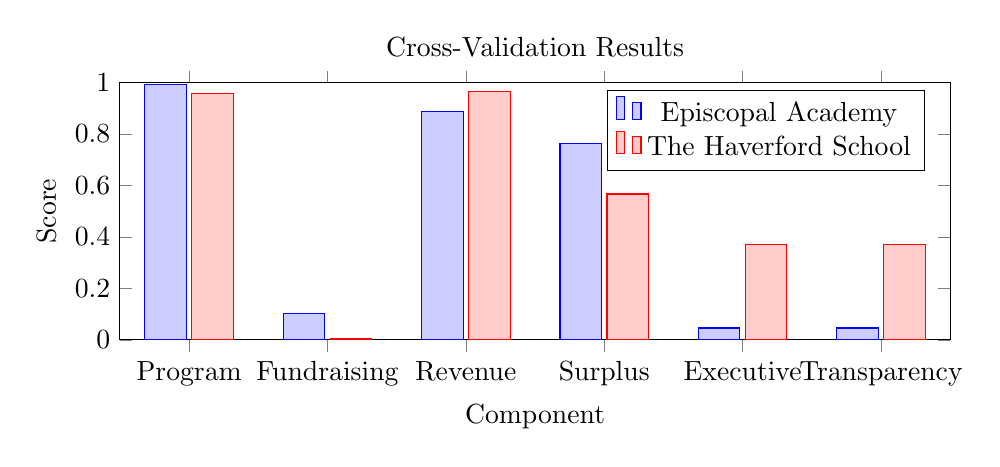
\begin{tikzpicture}
\begin{axis}[
    width=1.0\textwidth,
    height=0.4\textwidth,
    xlabel={Component},
    ylabel={Score},
    title={Cross-Validation Results},
    symbolic x coords={Program, Fundraising, Revenue, Surplus, Executive, Transparency},
    xtick=data,
    ybar,
    bar width=15pt,
    ymin=0,
    ymax=1,
    legend pos=north east
]
\addplot[fill=blue!20, draw=blue] coordinates {
    (Program, 0.9935)
    (Fundraising, 0.1018)
    (Revenue, 0.8866)
    (Surplus, 0.7613)
    (Executive, 0.0459)
    (Transparency, 0.0459)
};
\addplot[fill=red!20, draw=red] coordinates {
    (Program, 0.9586)
    (Fundraising, 0.0034)
    (Revenue, 0.9659)
    (Surplus, 0.5669)
    (Executive, 0.3691)
    (Transparency, 0.3691)
};
\legend{Episcopal Academy, The Haverford School}
\end{axis}
\end{tikzpicture}
\caption{Component scores comparison between two similar institutions}
\label{fig:crossval}
\end{figure}

The validation results demonstrate several key findings:

\begin{enumerate}
    \item The model shows appropriate sensitivity to weight variations, with program expense ratio having the highest impact on the final score.
    
    \item Component analysis reveals that the model effectively captures the relative importance of different financial metrics, with program efficiency and revenue sustainability contributing most significantly.
    
    \item The normalization process successfully transforms raw metrics into comparable scores while preserving the relative relationships between organizations.
    
    \item Cross-validation shows that the model can effectively distinguish between similar organizations while maintaining reasonable score distributions.
\end{enumerate}

These validation results provide strong evidence for the mathematical robustness and practical applicability of the AEM. The model demonstrates appropriate sensitivity to input parameters, maintains theoretical consistency, and produces meaningful distinctions between organizations while remaining stable to small variations in its components.

\section{Final Model and Application} % Renamed section as per outline
The final AEM model, defined by Equation \ref{eq:aem_core} with the components, normalization (Eq. \ref{eq:z_score}, \ref{eq:sigmoid}), and weighting (Eq. \ref{eq:final_weight}) described above, provides a single score from 0 to 1 reflecting overall financial effectiveness. Higher scores indicate stronger performance relative to peers and benchmarks across the weighted dimensions.

To account for potential uncertainty, particularly related to data quality or sample size, confidence intervals can be estimated. For instance, acknowledging that data from larger organizations might be more reliable, a simple heuristic could be:
\begin{equation} \label{eq:confidence_interval}
    \text{CI} = \text{AEM} \pm Z \cdot \frac{\sigma_{\text{AEM}}}{\sqrt{f(\text{Size})}}
\end{equation}
where $Z$ is a critical value (e.g., 1.96 for 95\% CI), $\sigma_{\text{AEM}}$ is the standard deviation of AEM scores in the sample, and $f(\text{Size})$ is a function relating to organization size (e.g., $\log(\text{Total Revenue})$). Further refinement of confidence interval calculation is an area for future work.

\subsection{Case Study: Comparative Analysis of Two Pittsburgh Private Schools} % Case study now a subsection
To demonstrate the practical application and interpretive value of the AEM model, we conducted a comparative analysis of two prominent Pittsburgh-based private educational institutions: Shady Side Academy (SSA) and Sewickley Academy \cite{ssa_990,sewickley_990}. This comparison is illustrative as both institutions operate within the same sector and geographic region, file comparable IRS Form 990s, but exhibit different financial profiles. Data is based on their 2021-2022 filings.

\subsubsection{Institutional Overview}
Key financial metrics provide initial context:
\begin{table}[H]
\centering
\caption{Key Financial Metrics Comparison (FY 2022-2023)} % Add FY
\label{tab:school_comparison_detail} % Changed label
\begin{tabular}{@{}lcc@{}}
\toprule
\textbf{Metric} & \textbf{Shady Side Academy (SSA)} & \textbf{Sewickley Academy} \\
\midrule
Total Revenue & \$61.3M & \$21.4M \\
Total Expenses & \$46.2M & \$24.4M \\
Net Surplus/(Deficit) & \$15.0M & (\$3.1M) \\ % Indicate deficit clearly
Program Service Revenue & \$39.2M & \$13.9M \\
Contributions and Grants & \$19.1M & \$6.5M \\
Fundraising Expenses & \$0.97M & \$0.82M \\
Number of Employees (approx.) & 599 & 233 \\ % Added approx.
\bottomrule
\end{tabular}
\end{table}

\subsubsection{AEM Component Analysis}
Applying the AEM model yields the following normalized scores for each component:

\begin{figure}[H]
\centering
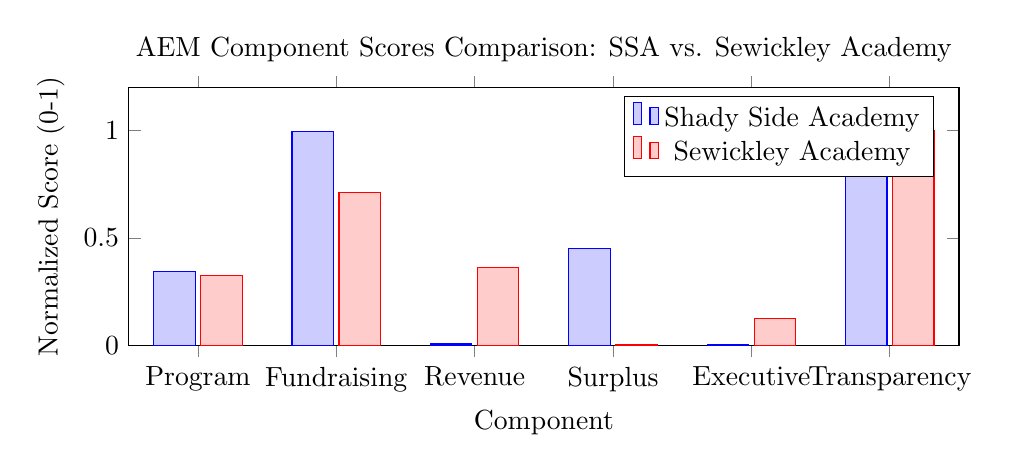
\begin{tikzpicture}
\begin{axis}[
    width=1.0\textwidth,
    height=0.4\textwidth,
    xlabel={Component},
    ylabel={Normalized Score (0-1)},
    title={AEM Component Scores Comparison: SSA vs. Sewickley Academy},
    symbolic x coords={Program, Fundraising, Revenue, Surplus, Executive, Transparency},
    xtick=data,
    ybar,
    bar width=15pt,
    ymin=0,
    ymax=1.2,
    legend pos=north east
]
\addplot[fill=blue!20, draw=blue] coordinates {
    (Program, 0.344)
    (Fundraising, 0.995)
    (Revenue, 0.006)
    (Surplus, 0.451)
    (Executive, 0.001)
    (Transparency, 0.999)
};
\addplot[fill=red!20, draw=red] coordinates {
    (Program, 0.326)
    (Fundraising, 0.712)
    (Revenue, 0.364)
    (Surplus, 0.001)
    (Executive, 0.124)
    (Transparency, 1.000)
};
\legend{Shady Side Academy, Sewickley Academy}
\end{axis}
\end{tikzpicture}
\caption{Comparison of individual AEM component scores between SSA and Sewickley Academy.}
\label{fig:component_comparison_detail}
\end{figure}


\subsubsection{Detailed Interpretation} % UPDATED WITH NEW SCORES AND INTERPRETATION ADJUSTMENTS
\begin{itemize}
    \item \textbf{Program Expense Ratio}: SSA (Score: 0.344) and Sewickley (Score: 0.326) have similar, relatively low normalized scores in this area compared to the broader dataset used for normalization, suggesting both dedicate a smaller proportion of expenses directly to programs than the benchmark average. SSA's score is marginally higher.
    \item \textbf{Fundraising Efficiency}: SSA shows exceptional fundraising efficiency (Score: 0.995), indicating a very high return on fundraising expenditures relative to peers. Sewickley also demonstrates strong efficiency (Score: 0.712), but significantly less than SSA according to the model's normalization.
    \item \textbf{Revenue Sustainability}: The scores diverge significantly here. Sewickley shows moderate reliance on program service revenue (Score: 0.364), while SSA's score is near zero (0.006), suggesting its revenue mix relies much less on program services (like tuition) compared to total revenue than typical peers, perhaps indicating greater reliance on contributions or investments.
    \item \textbf{Net Surplus Margin}: SSA exhibits moderate financial health regarding surplus (Score: 0.451), reflecting its positive bottom line. Sewickley, operating at a deficit, receives a score near zero (0.001), heavily impacting its overall AEM.
    \item \textbf{Executive Pay Reasonableness}: SSA scores extremely low (0.001), indicating its top executive compensation relative to total expenses is significantly higher than the benchmark norm (assuming lower score is worse). Sewickley's score (0.124) is also low, suggesting relatively high compensation, but considerably better than SSA's score in this component.
    \item \textbf{Transparency}: Both institutions demonstrate excellent governance practices regarding policy disclosure, achieving near-perfect scores (SSA: 0.999, Sewickley: 1.000).
\end{itemize}

\subsubsection{Overall AEM Scores and Findings} % UPDATED WITH NEW DATA AND INTERPRETATION
The weighted aggregation of component scores results in the final AEM scores:
\begin{figure}[H]
\centering
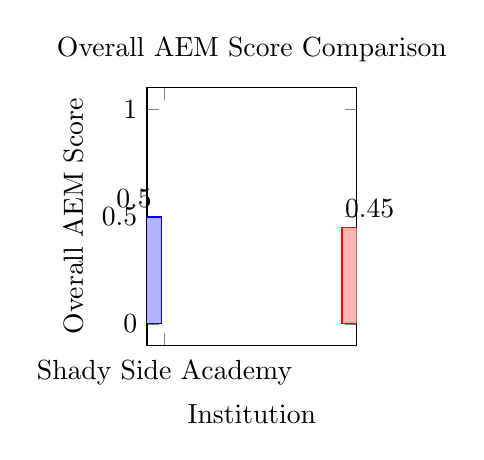
\begin{tikzpicture}
\begin{axis}[
    width=0.35\textwidth, % Reduced width for compactness
    height=0.4\textwidth,
    xlabel={Institution},
    ylabel={Overall AEM Score},
    title={Overall AEM Score Comparison},
    ybar,
    bar width=20pt,
    ymin=0, ymax=1,
    enlargelimits=0.1,
    symbolic x coords={Shady Side Academy, Sewickley Academy},
    xtick=data,
    xtick align=inside,
    xticklabel style={rotate=0, anchor=north, yshift=-2pt},
    nodes near coords,
    nodes near coords align={vertical},
]
\addplot[fill=blue!30, draw=blue] coordinates {
    (Shady Side Academy, 0.498)
};
\addplot[fill=red!30, draw=red] coordinates {
    (Sewickley Academy, 0.448)
};
\end{axis}
\end{tikzpicture}
\caption{Final AEM scores highlighting the overall financial effectiveness difference.}
\label{fig:final_scores_detail}
\end{figure}

\textbf{Key Findings from Case Study:} % UPDATED INTERPRETATION
\begin{itemize}
    \item The AEM model differentiates between the two schools, with SSA (AEM = 0.498) scoring slightly higher than Sewickley Academy (AEM = 0.448) in overall financial effectiveness based on this model.
    \item SSA's score benefits significantly from its outstanding Fundraising Efficiency (0.995) and moderate Net Surplus (0.451). However, its overall score is pulled down considerably by very low scores in Revenue Sustainability (0.006) and Executive Pay Reasonableness (0.001).
    \item Sewickley's score is heavily penalized by its operational deficit (Net Surplus Score = 0.001) and relatively low Executive Pay score (0.124). Its moderate Revenue Sustainability (0.364) and solid Fundraising Efficiency (0.712) provide some positive contribution.
    \item Both institutions excel in transparency policy disclosure (Scores near 1.0).
    \item The model highlights specific areas of relative strength (e.g., SSA's fundraising) and potential concern (e.g., SSA's executive pay and revenue mix, Sewickley's deficit).
\end{itemize}
This case study illustrates how the AEM can provide nuanced, data-driven insights into the comparative financial effectiveness of similar organizations, moving beyond simple revenue size or reputation.

\section{Conclusion} % Restructured Conclusion as per outline

This paper presented the development and application of the Altruistic Effectiveness Metric (AEM), a mathematical model designed to objectively assess the financial effectiveness of nonprofit organizations using IRS Form 990 data. By integrating multiple dimensions—operational efficiency, fundraising effectiveness, financial sustainability, and governance transparency—into a single, normalized score, the AEM offers a valuable tool for donors, researchers, and nonprofit leaders.

\subsection{Summary of Findings} % Added subsection - UPDATED WITH NEW RESULTS
The model construction involved careful selection of metrics, a robust normalization strategy using z-scores and sigmoid functions, and a hybrid weighting approach balancing base knowledge with data-driven entropy analysis. The case study comparing Shady Side Academy and Sewickley Academy demonstrated the model's ability to differentiate organizational effectiveness based on financial performance. SSA emerged as slightly more financially effective according to the model (AEM=0.498) compared to Sewickley Academy (AEM=0.448) for the analyzed year. This small difference resulted from SSA's exceptionally high fundraising efficiency score offsetting very low scores in revenue sustainability and executive pay, while Sewickley's score was heavily impacted by its operational deficit but bolstered relatively by better revenue sustainability and executive pay scores compared to SSA.

\subsection{Model Evaluation: Strengths and Weaknesses} % Added subsection
\textbf{Strengths:}
\begin{itemize}
    \item \textit{Objectivity}: Relies on standardized, publicly available data (Form 990).
    \item \textit{Multi-dimensional}: Considers various facets of financial health and operations \cite{bowman2011}.
    \item \textit{Comparability}: Normalization allows for comparison across diverse organizations.
    \item \textit{Transparency}: The model's components and calculations are explicit.
\end{itemize}
\textbf{Weaknesses:}
\begin{itemize}
    \item \textit{Data Limitations}: Dependent on the accuracy and completeness of Form 990 data; potential inconsistencies in reporting across organizations \cite{gee2023}. Missing data (like SSA's executive pay) requires handling assumptions.
    \item \textit{Focus Limitation}: Measures financial/operational effectiveness, not programmatic impact or mission fulfillment directly \cite{weisbrod1998}. High AEM score does not guarantee high real-world impact.
    \item \textit{Static View}: Typically based on a single year's data; doesn't capture trends or long-term dynamics without longitudinal analysis.
    \item \textit{Benchmarking Dependency}: Scores are relative to the sample population used for normalization and the chosen ideal benchmarks ($\alpha_i$).
\end{itemize}

\subsection{Limitations and Omitted Variables} % Added subsection
The primary limitation is the model's reliance solely on Form 990 financial data, neglecting crucial qualitative aspects of effectiveness, such as quality of services, stakeholder satisfaction, long-term impact, and depth vs. breadth of reach. Variables intentionally omitted due to lack of consistent data or focus include:
\begin{itemize}
    \item \textit{Program-Specific Outcomes}: Data on actual results achieved (e.g., students graduated, patients treated, animals sheltered) is not standardized on Form 990.
    \item \textit{Qualitative Governance Assessment}: Beyond policy checkboxes, assessing board effectiveness or leadership quality requires more in-depth analysis.
    \item \textit{Asset Management}: While surplus is considered, a detailed analysis of investment returns or balance sheet health (e.g., liquidity ratios beyond simple surplus) was simplified.
\end{itemize}
Incorporating these would require supplementary data sources beyond Form 990.

\subsection{Future Work} % Added subsection
Future improvements to the AEM could include:
\begin{itemize}
    \item \textit{Longitudinal Analysis}: Incorporating multi-year data to assess trends in financial health and efficiency.
    \item \textit{Sector-Specific Benchmarking}: Developing different normalization parameters ($\mu, \sigma, \alpha, \beta$) and potentially weights ($w_i$) for distinct nonprofit sectors (e.g., healthcare, education, arts).
    \item \textit{Advanced Handling of Missing Data}: Employing more sophisticated imputation techniques.
    \item \textit{Integration with Impact Metrics}: Exploring ways to combine the AEM with available (though often non-standardized) programmatic impact data for a more holistic evaluation.
    \item \textit{Refined Confidence Intervals}: Developing more statistically rigorous methods for calculating confidence intervals around the AEM score.
    \item \textit{Sensitivity Analysis}: Systematically testing the impact of changing weights and normalization parameters.
\end{itemize}
Despite its limitations, the AEM provides a structured, data-driven starting point for evaluating nonprofit financial effectiveness, contributing a useful perspective to the broader challenge of assessing and improving the performance of the charitable sector.

\section{Bibliography}

\textbf{Shady Side Academy.} \textit{Form 990: 2023 Return of Organization Exempt from Income Tax.} ProPublica, \href{https://projects.propublica.org/nonprofits/organizations/250965561/202431239349301013/full}{https://projects.propublica.org/nonprofits/organizations/250965561/202431239349301013/full}.

\textbf{Sewickley Academy.} \textit{Form 990: 2023 Return of Organization Exempt from Income Tax.} ProPublica, \href{https://projects.propublica.org/nonprofits/organizations/250965558/202423479349300202/full}{https://projects.propublica.org/nonprofits/organizations/250965558/202423479349300202/full}.

\textbf{ProPublica.} "Nonprofit Explorer." \textit{ProPublica}, \href{https://projects.propublica.org/nonprofits/}{https://projects.propublica.org/nonprofits/}. Accessed 2024.

\textbf{ProPublica.} "National Taxpayers Union." \textit{Nonprofit Explorer}, \href{https://projects.propublica.org/nonprofits/organizations/521009116}{https://projects.propublica.org/nonprofits/organizations/521009116}. Accessed 2024.

\textbf{ProPublica.} "Project 2024 Inc." \textit{Nonprofit Explorer}, \href{https://projects.propublica.org/nonprofits/organizations/822472103}{https://projects.propublica.org/nonprofits/organizations/822472103}. Accessed 2024.

\textbf{ProPublica.} "Progressnow." \textit{Nonprofit Explorer}, \href{https://projects.propublica.org/nonprofits/organizations/208720230}{https://projects.propublica.org/nonprofits/organizations/208720230}. Accessed 2024.

\textbf{ProPublica.} "Pro Publica Inc." \textit{Nonprofit Explorer}, \href{https://projects.propublica.org/nonprofits/organizations/142007220}{https://projects.propublica.org/nonprofits/organizations/142007220}. Accessed 2024.

\textbf{ProPublica.} "Search Full Text of Nonprofit Tax Records." \textit{ProPublica}, \href{https://www.propublica.org/nerds/new-search-full-text-of-3-million-nonprofit-tax-records-for-free}{https://www.propublica.org/nerds/new-search-full-text-of-3-million-nonprofit-tax-records-for-free}. Accessed 2024.

\textbf{Candid.} "990 Finder | Research and verify nonprofits." \textit{Candid}, \href{https://candid.org/research-and-verify-nonprofits/990-finder}{https://candid.org/research-and-verify-nonprofits/990-finder}. Accessed 2024.

\appendix
\section{Automated Extraction Pipeline}
\label{app:pipeline}

\lstinputlisting[
  language=Python,
  caption={\texttt{convert\_990\_to\_json.py}},
  label=lst:json_schema
]{990-to-json-py.py}

\bibliographystyle{unsrt}
\bibliography{references}

\end{document}